%!TEX root = D2.1_AMIDSTModellingFramework.tex

\newpage
\newpage
\newcommand{\X}{\mathbf{X}}
\newcommand{\Y}{\mathbf{Y}}
\newcommand{\Z}{\mathbf{Z}}
\newcommand{\x}{\mathbf{x}}
\newcommand{\y}{\mathbf{y}}
\newcommand{\z}{\mathbf{z}}
\newcommand{\argmax}[1]{\underset{#1}{\operatorname{arg}\,\operatorname{max}}\;}


\subsection{Cajamar models}\label{Section:CajamarModels}
\label{Section:CajaMarModels}

There are two tasks to be solved for Cajamar's Use Case~\cite{Fer14b}. The main one is the estimation of the \emph{probability of default}, defined as the probability that a customer will end up as defaulter at any time within the next two years. The second task consists in obtaining good customer profiles in terms of risk, so that marketing campaigns can be specifically targeted to these low risk customers. 

\subsubsection{State-of-the-art of the application scenarios} \label{SubSection:}

This section is devoted to explaining what are the current Cajamar approaches to solve the risk prediction and the profile extraction problems. Thus, it will be clear which are the expected contributions of our project and also the point to start from.

In any commercial bank, every time a customer applies for a loan, the bank experts evaluate the customer's risk profile
before making their decision. At Cajamar, this risk evaluation protocol is performed by estimating whether the client is
going to default or not within the following two years\footnote{When a client is labelled as defaulter, he/she will
  remain as defaulter in the database at least for one more year. Then, the client could become non-defaulter again when
  his/her debts has been appropriately paid during the last year.}. The problem of predicting the risk of default is
currently solved at Cajamar by an automatic supervised classification model (a logistic regression model). It takes
information about the recent financial activity of a customer, as well as information about recent past payment
behaviors provided by other Spanish financial institutions. Finally, using this collected information, the probability
that the client will default during the following two years is computed. The procedure currently employed for this has
some limitations. First, the model does not assume any dependences among the variables. Second, current predictions are
made using only $27$ variables out of the more than $1000$ variables available, which might mean that useful information is being discarded. Finally, updates in risk predictions are made on a monthly basis, whereas the predictive model is only updated after several years. These low update frequencies are partly due to limitations in the available commercial software and the computing resources.

Regarding the profile extraction problem, the marketing department periodically launches marketing campaigns for the
recruitment of new products by existing customers (i.e., a new credit card, an insurance, etc.). The success of these
campaigns depends greatly on the client group to which the campaign is targeted. It is also crucial to reduce as much as
possible unnecessary expenses focused on non-potential customers.  For this purpose, the marketing group currently
proceed as follows. Using their own marketing models, and in collaboration with the risk department\footnote{Note that,
  expert knowledge has currently an important relevance for this task.}, they provide some restrictions over a subset of
variables to be satisfied by the targeted clients. For instance, they must all be older than 60 or the annual incomes must be higher than $30.000$ euros. In this way they conform the group of clients taking part in the campaign. The main limitation of this approach is that a detailed analysis shows that non-solvent clients (i.e. clients with high probability of defaulting) are also included as part of the campaign, revealing the weakness of the process and the resulting economic losses. The refinement of this final group of clients will be the main challenge of our proposal. 


%-------------------------------------------------------------------------------------------------------
\subsubsection{Predicting probability of default} \label{SubSection:Predicting}
%-------------------------------------------------------------------------------------------------------

Our objective is to tackle the current limitations of the risk prediction problem by \textit{daily} learning the predictive model and also updating the risk of default for every bank customer. Dependences among the variables will now be considered, as well as including all the variables in the analysis. With these changes, Cajamar plans to improve the quality of the prediction model by increasing the area under ROC curve significantly.


Therefore, the process will consist in building a \textit{training set} as well as the set of customers to be evaluated, called \textit{evaluation set} (see~\cite{Fer14b}). How these data sets are generated gives us some insights into the nature of this risk prediction problem (see Figure~\ref{Figure:CajaMarTimeLine} for a better understanding):

%Next, we detail how these data sets are collected .
%Figure~\ref{Figure:CajaMarTimeLine} illustrates how both evaluation and training data sets are collected within a time-line. The current time is denoted as $t$ and the time $2$ years back as $k$, i.e., $k=t-2$ years. 

\begin{figure}[ht!]
\centering
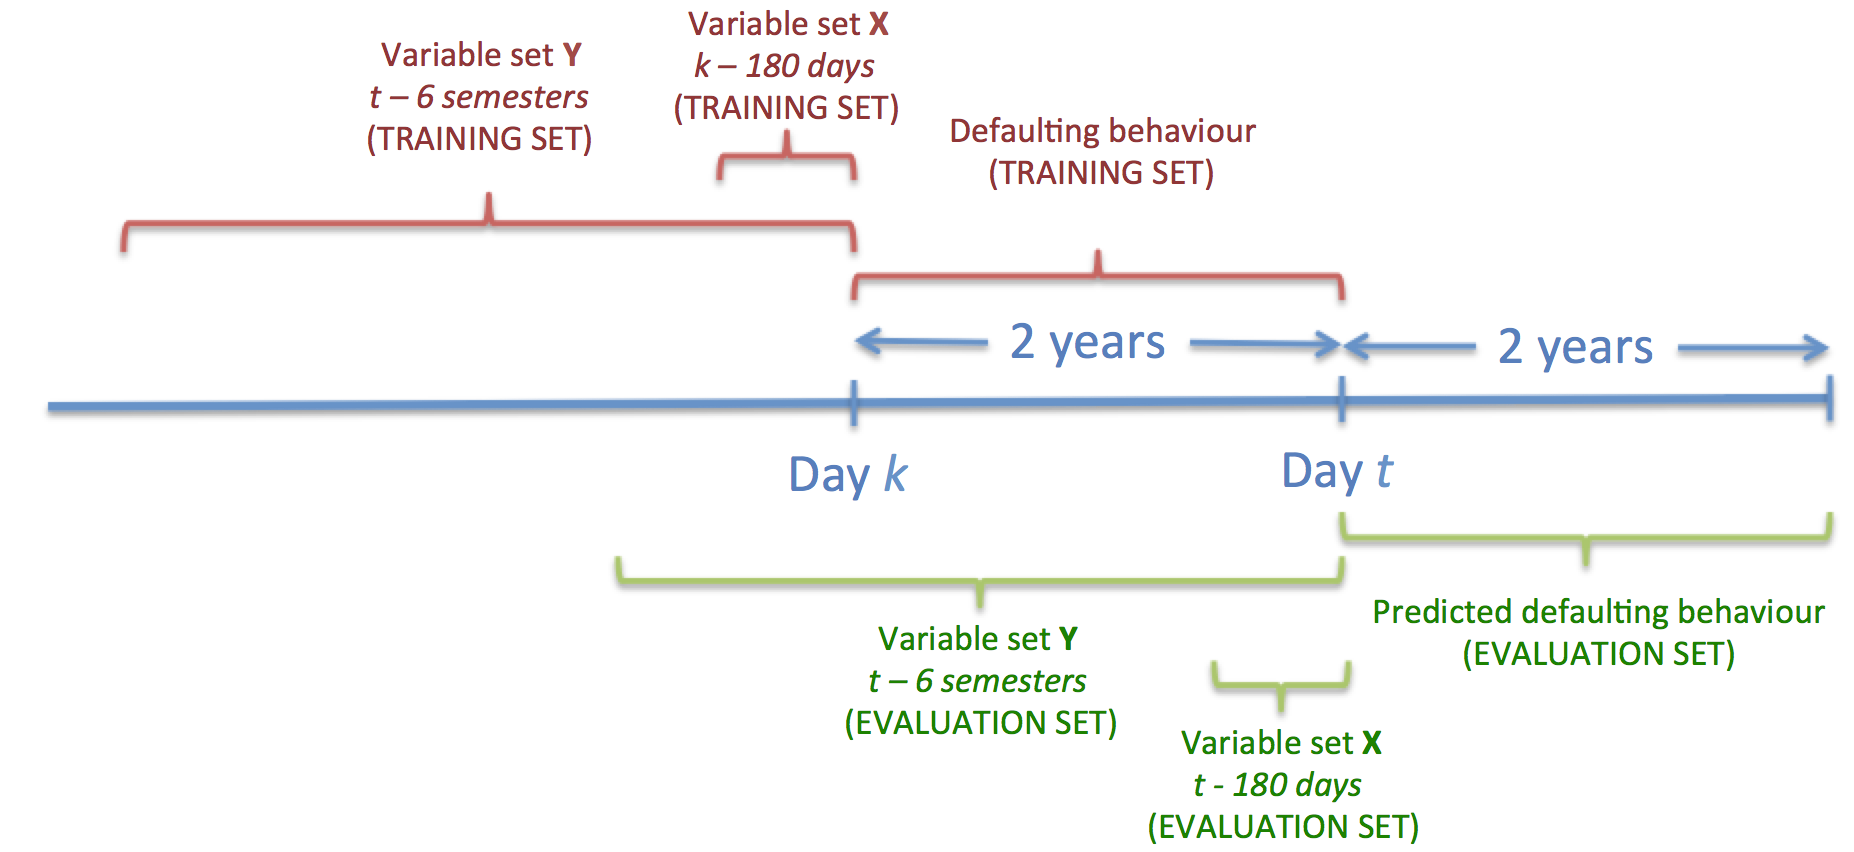
\includegraphics[scale=0.45]{figures/CajaMarTimeLine}
\caption{\label{Figure:CajaMarTimeLine}Time-line showing the generation of the evaluation (in green) and training (in red) data sets. $t$ refers to the present time and $k$ corresponds to time $t-2$\ years. Both in the training and test data sets, there are two disjoint groups of variables, denoted as $\X$ and $\Y$, with different past information considered, $180$ days back (daily) and $6$ semesters back (by semester), respectively.}

\end{figure}

\begin{itemize}

\item \textbf{Model evaluation data set:} This data is created at time $t$ and contains a record for every client to be evaluated. Note that information about the predicted defaulting behaviour is missing at time $t$ and it will be obtained after performing inference on the model. Predictive variables refer here to the financial activity and payment behaviour of the customers in recent past as well as to their socio-demographic information which usually does not change over time. 

There are attributes, denoted as $\X$, for which information during the last 180 days is considered. 
%recent \textcolor{red}{{\bf financial activity}}of a customer refers to attributes such as ``account balance'', ``number of credit card operations'', etc. stored in the last 180 days. 
These attributes usually change daily for a customer, so they are encoded by introducing a set of variables for each attribute, one for each day back from the current time $t$. Hence, the financial activity of a customer is specified by a number of variables equal to 180 times the number of attributes. For others attributes, denoted as $\Y$, we are interested in information from the last $36$ months grouped by semester. 
%In the case of \textcolor{red}{{\bf past payment behaviour}}, the attributes refer to variables related to \textcolor{red}{payments inside Cajamar (loans, mortgages, credits, etc.).} Information from the last 36 months grouped by semester is considered for these variables. 
Therefore, similar to previous group of variables, $6$ variables for each of these attributes will be considered. Finally, there are some other static variables, denoted as $\Z$, not included in Figure~\ref{Figure:CajaMarTimeLine} as they are not indexed over time. The data set for the evaluation of customers is depicted in Table~\ref{tab:EvaluationDataset}. 


%with information about \textcolor{red}{payments to other financial institutions or companies (phone and electricity bills, public bodies, etc.)} 
%are included in this group of variables. They are denoted as .

%The group of variables denoted as $\Z$ mainly includes socio-demographic variables and they are not indexed over time as they remain fixed.  

\begin{table}[ht!]
\centering
\begin{tabular}{c|ccc|ccc|c}
	&\multicolumn{3}{c|}{Days} & \multicolumn{3}{c|}{Semester} \\
     Time $t$              & $\X^{(t-180)}$ & $\ldots$ & $\X^{(t-1)} $ & $\Y^{(t-6)}$  & $\ldots$ & $\Y^{(t-1)} $ & $\Z$  \\  
\hline
Client$_1$  &                                                  &              &                     &                               &                     &        \\ 
$\vdots$      &                                                 &               &                     &                                &                     &      \\ 
Client$_n$  &                                                &               &                     &                                &                     &     \\ 
\end{tabular}
\caption{Evaluation data set at time $t$ for all the clients. Three groups of attributes $\X$, $\Y$ and $\Z$ are distinguished according to the past information required. Current time is denoted as $t$.}
\label{tab:EvaluationDataset} 
\end{table}

Thus, the objective is to compute the probability of defaulting within the following two years of each record from the evaluation data set, and afterwards update the risk table in the system (see Table~\ref{tab:riskTable}).

\begin{table}[ht!]
\centering
\begin{tabular}{c|ccc|ccc|c}
     Time $t$  & Risk of being defaulter \\  
\hline
Client$_1$  &    $r_1$  \\ 
$\vdots$      &   $\vdots$   \\ 
Client$_n$  &   $r_n$  \\ 
\end{tabular} 
\caption{Risk table for the bank customers where $r_i$ represents the probability of being defaulter for customer $i$.}
\label{tab:riskTable}
\end{table}

If, at some point, the probability of default of a customer rises above a predefined threshold, the bank may take preventive actions to reduce the risk of defaulting by this customer.


\item \textbf{Model training data set:}  This data set is also built at time $t$ in a similar way as the evaluation data. It contains the same set of features as well as the target variable \textit{Defaulter} but with information referred to time $k$ instead (two years back). Note that, at time $t$, we have information of the \textit{Defaulter} variable in the period of time from $k$ to $t$. Thus,  Defaulter$^{(k)}$ indicates if at some point in this period she/he was a defaulter.

The data set for training/updating the model is depicted in Table~\ref{tab:TrainingDataset}.
\begin{table}[ht!]
\centering
\begin{tabular}{c|ccc|ccc|c|c}
	&\multicolumn{3}{c|}{Days} & \multicolumn{3}{c|}{Semester} & \\
     Time $t$              & $\X^{(k-180)}$ & $\ldots$ & $\X^{(k-1)} $ & $\Y^{(k-6)}$  & $\ldots$ & $\Y^{(k-1)} $ & $\Z$ & Defaulter$^{(k)}$\\  
\hline
Client$_1$  &                                                  &              &                     &                               &                     &        &  \\ 
$\vdots$      &                                                 &               &                     &                                &                     &       & \\ 
Client$_n$  &                                                &               &                     &                                &                     &     & \\ 
\end{tabular} 
\caption{Training data set built at time $t$ with $k=t - 2$ years.  The notation for predictive variables is the same as in Table~\ref{tab:EvaluationDataset}.}
\label{tab:TrainingDataset} 
\end{table}

Table~\ref{tab:TrainingDataset} shows the training data set where each record contains the values for all predictive variables and a class value labelled as \emph{non-defaulter} only when there is no evidence of defaulting in the period from $k$ to $t$ (2 years). 

\end{itemize}



In what follows, we propose two modelling solutions for the risk prediction problem: static and dynamic.

%-------------------------------------------------------------------------------------------------------
\subsubsection*{Static model} 
%-------------------------------------------------------------------------------------------------------

In this first approach we do not explicitly consider some of the dynamics of the problem, meaning that we do not model that a customer can be non-defaulter and defaulter at different times (e.g., a customer can be creditworthy and, after some time, go bankrupt due to unemployment). Instead, we consider a static model that predicts whether the client will default or not within the next 2 years based on the financial behaviour of the client over a recent past. This is in fact similar to the current Cajamar prediction system. Note that any dynamic model should be at least as good as the static one. 

Figure~\ref{Figure:CajaMarStatic} shows the general structure of the static model. The notation for predicting variables are the same as in previous section. Note that attributes in groups $\X$ and $\Y$ may be duplicated over the time creating the corresponding set of variables. 

\begin{figure}[ht!]
  \centering
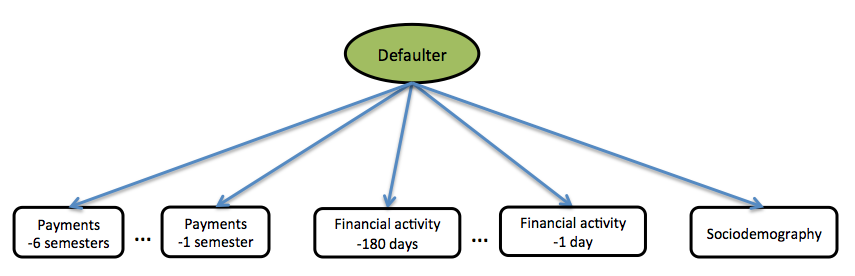
\includegraphics[scale=0.5]{./figures/CajaMarModel0}
\caption{\label{Figure:CajaMarStatic}Global structure of the static model. Each white box represents a set of variables for a particular time. The green node on top is the class variable \emph{Defaulter}, that represents the probability that a customer will default within the next two years. } 
\label{fig:CajamarStaticModel}
\end{figure}

According to expert knowledge from the bank, the predictive variables (mainly those within each white box) are expected to be related. Thus, in a first attempt we are assuming that only variables within each white box can be connected (e.g., according to a tree structure).

Another issue to consider, is the possibility that one variable is a replica or contain similar information than another variable, something likely to be encountered in Cajamar data. Consequently, their joint contribution will not only make learning and inference computationally more expensive, but it may also lead to a worse performance. This justifies the need to explore and use suitable feature selection techniques as specified in Use Case 2 of Cajamar Requirement analysis~\cite{Fer14b}.

It is also of major interest to analyse the type of probability distributions to use in the proposed model. Figure \ref{Figure:cajamarMixt} shows the histograms for the values of one continuous predictive variable conditioned to defaulter (left curve) and non-defaulter (right curve) respectively. The resulting density curves represent a credible approximation using mixture of Gaussian distributions, which is the case for most of the remaining predictive variables. Note that, for defaulters, the values of this variable are overall lower compared to those corresponding to non-defaulters.

\begin{figure}[ht!]
  \centering
    \begin{tabular}{cc}
    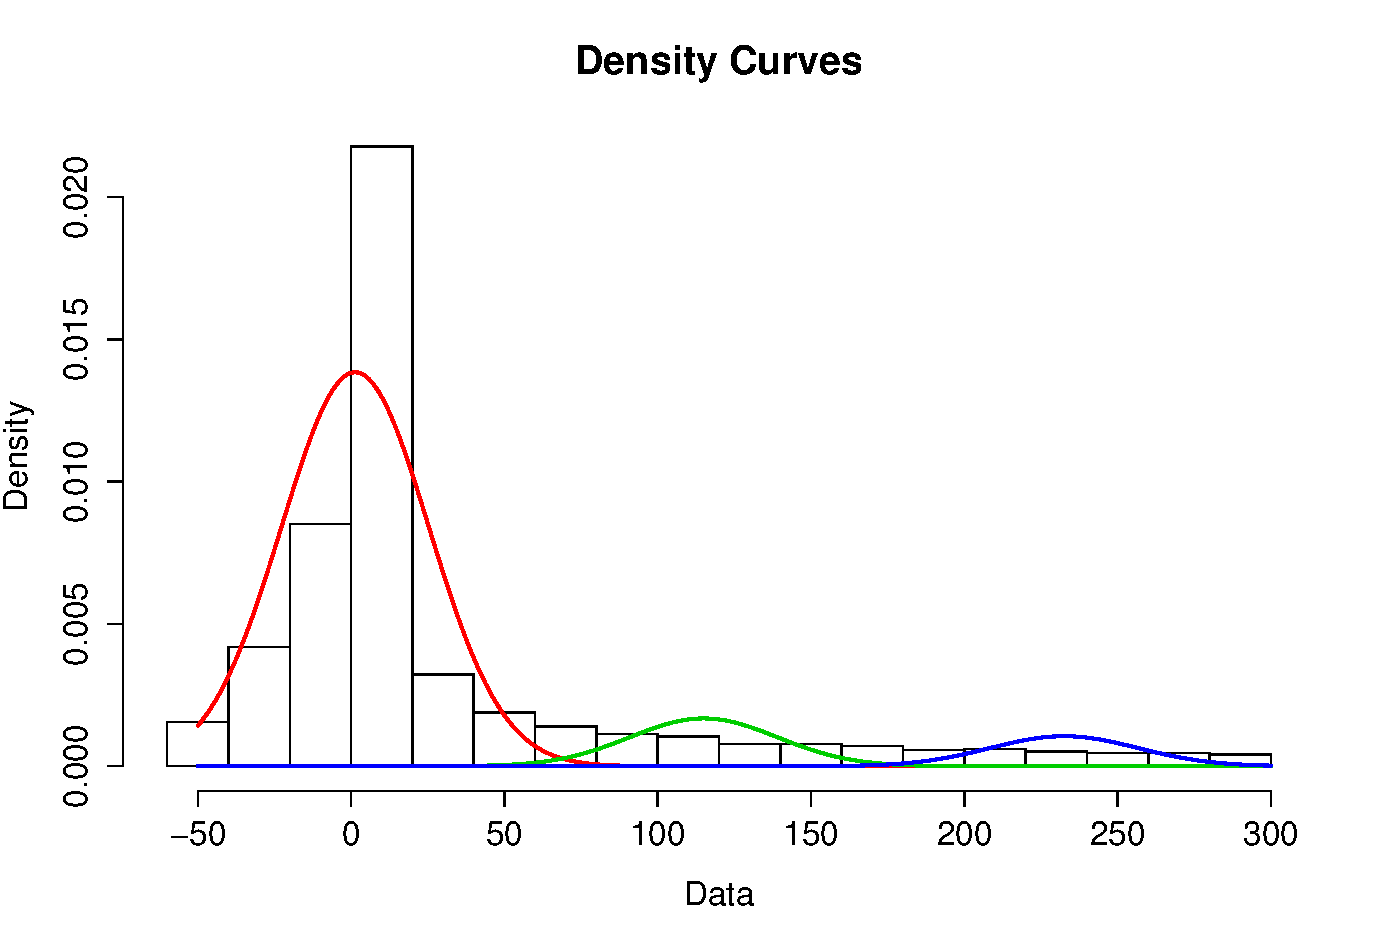
\includegraphics[width=70mm]{figures/CajaMarmixtureBalanceDef}&
    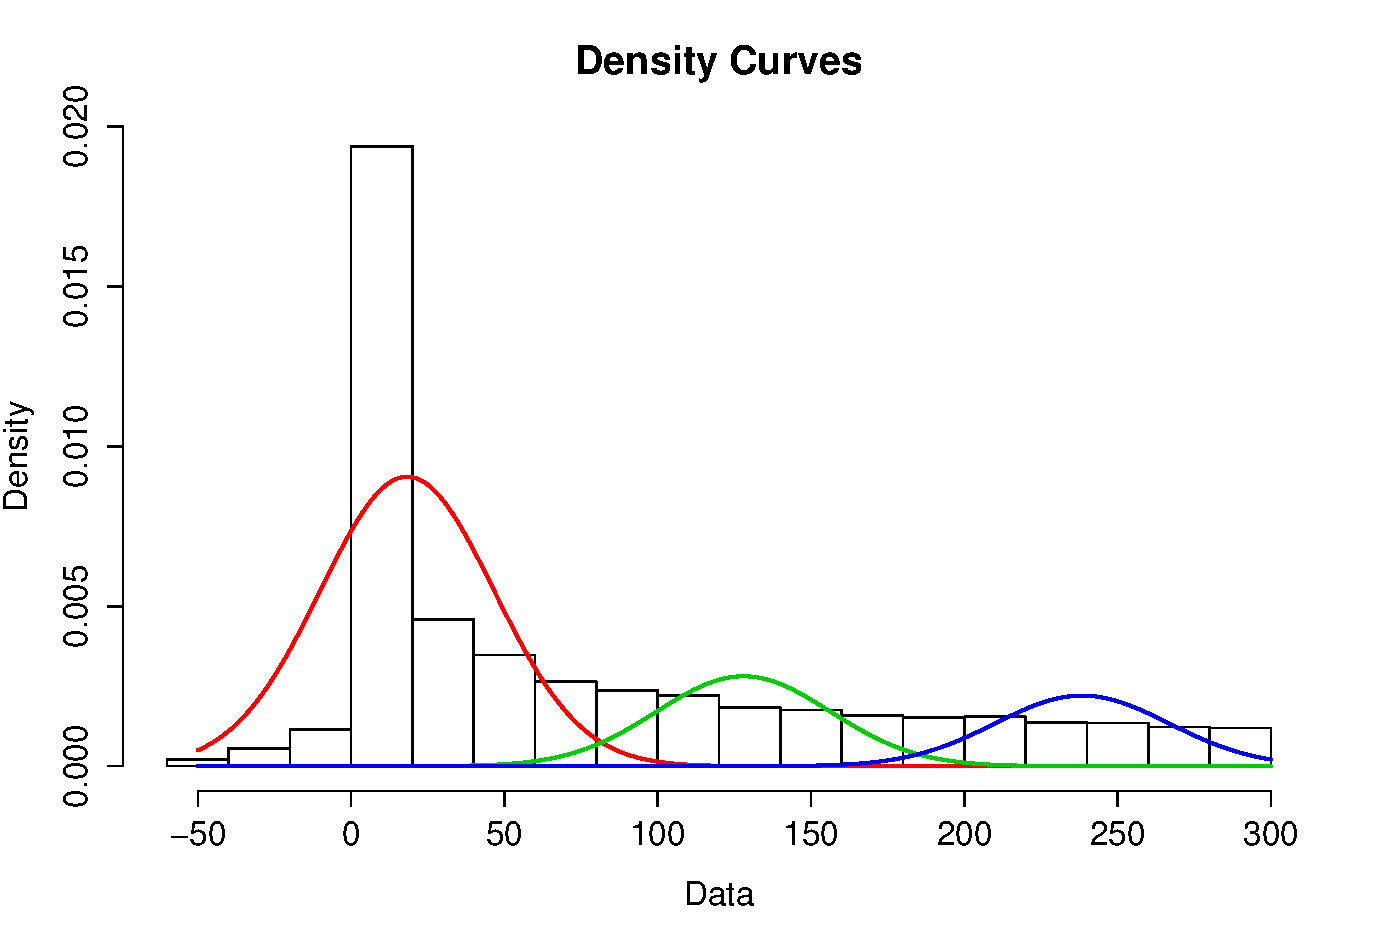
\includegraphics[width=70mm]{figures/CajaMarmixtureBalanceNonDef}\\
  \end{tabular}
    \caption{\label{Figure:cajamarMixt}Mixture of Gaussian approximations of one predictive variable conditioned to the class variable values defaulter (left) and non-Defaulter (right).}
\end{figure}

There exist however discrete (non-ordinal) predictive attributes which impose a limitation in the structure of the conditional Gaussian network, since discrete attributes cannot have continuous parents, as pointed out in Section~\ref{SubSection:HybridBNs}. 
%However, this might not be a problem for the semi-naive Bayesian network to be considered, and it is certainly not a problem for naive Bayes. 
Although, this might not be a problem for some Bayesian network structures, if this limitation were found to be problematic, then other probability distributions families will be explored, such as Mixture of Truncated Basis Functions~\cite{Langseth12}, which can cope with any generic model structure. 

In summary, the process of building the static model and updating the customers' risk consists of the following steps:

\begin{enumerate}
\item Construct, every day, a single flat table containing the information for model training (see Table~\ref{tab:TrainingDataset}) using a set of SQL queries over the main relational data set. Note that, for instance, for the variables set $\X$, training data between two consecutive days $t$ and $t+1$ only differ in the new data arriving at day $t+1$ and obviating the data 180 days back from day $t$. A similar idea is applied for the set $\Y$.
\item Update the existing BN classifier with the new data. If the underlying probability distributions belong to the exponential family, this step will be made incrementally by updating the sufficient statistics of the variables. Otherwise, the model must be learnt from scratch. Although relationships are more common between variables within each box, dependences among variables in different boxes could be also considered. This possibility is tackled in Section~\ref{subsubsec:CajamarDiscussion}.
\item Construct a single flat table with the latest information about customers (evaluation data set as depicted in Table~\ref{tab:EvaluationDataset}) in order to compute the latest risk profiles. 
\item Update the risk in Table~\ref{tab:riskTable} for every customer by propagating each record from the evaluation data set on the static BN classifier obtained in Step 2.
\end{enumerate}

%-------------------------------------------------------------------------------------------------------
\subsubsection*{Dynamic model} 
%-------------------------------------------------------------------------------------------------------

In this second approach, we will consider the dynamic structure of the problem, since the behaviour of the customers evolves over time (e.g., the account balance is continuously changing from one month to another, the incomes, etc.) as well as their class labels either defaulters or non-defaulters (e.g., customers can be creditworthy and, after some time, go bankrupt because they have lost their job). 

Figure~\ref{fig:global_temp} represents the global idea of the proposed dynamic model. Each of the defaulter variable at different times represents whether a customer will default in the following 2 years from $t$. 

The previous model can be compactly represented by a DBN made of components as the one displayed in 
Figure~\ref{fig:component}. Next, we detail the meaning of each node.

Defaulter$_{t+1}$ represents the class variable at time slice $t+1$, i.e., being defaulter or non-defaulter within the next two years, and depends on class variable Defaulter$_{t}$ at time $t$ considering a first Markov order. Each feature variable in ${\bf X}_t$ with a clear dynamic component at time $t$, is linked to the same variable in ${\bf X}_{t+1}$ at time $t+1$. Although this is a reasonable assumption for most of the variables, this first Markov order relationship however might prove insufficient for some of the variables. Figure~\ref{fig:CajamarCorrelogramsAndPartial} shows a correlogram (left) and a partial  correlogram (right) for a continuous predictive variable (see Section~\ref{Section:Preliminaries}). The partial correlogram drops to almost zero for a lag equal to $2$, making a first Markov order assumption reasonable for this specific variable. However, a higher order might be necessary for other variables, meaning that, for an order 2 for instance, sample from time $t-2$ still could have an influence on the current sample at time $t$ given the one at time $t-1$. Similar reasoning is applied for an order higher than 2.  

To this end, variables in $\bar{{\bf X}}_{t-1}$ and $\bar{\bf{X}}_{t}$ represent memory variables at time $t$ and $t+1$ respectively. The inclusion of this type of variables might be necessary when we have evidence that first order Markov relationships do not hold and we need to account for information coming from the past. Memory variables representing averaged or accumulated values both during the last $180$ days, could, for instance, capture these past dependences. Another reason to include these memory variables is that, even though they are computed from others, they provide information that might be disperse in the data and hardly can be captured by other variables as a whole. Moreover, the use of memory variables avoids building complex dynamic models with high Markov orders. In principle, memory variables in $\bar{{\bf X}}_{t-1}$ and $\bar{{\bf X}}_{t}$ are not connected over time, as their dynamic component is partially captured through the dynamic variables ${\bf X}_{t}$ and ${\bf X}_{t+1}$.


\begin{figure}[htbp]
\begin{center}
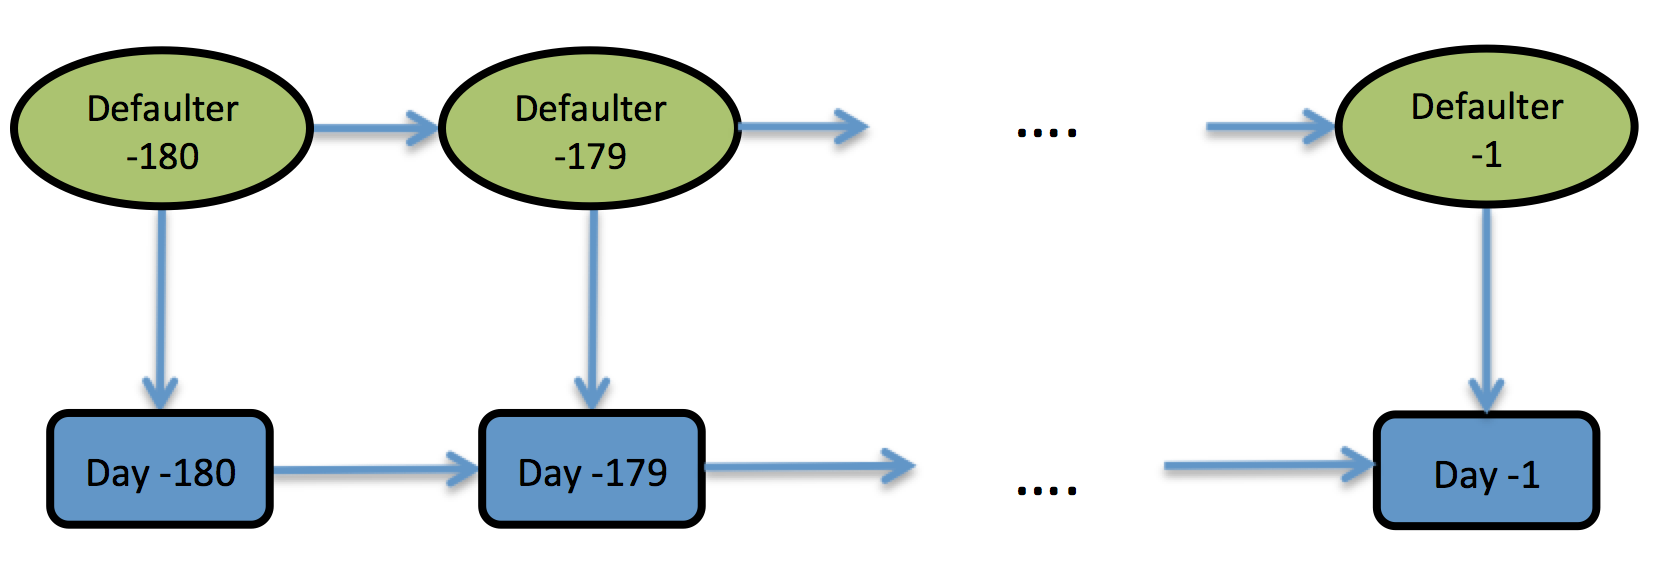
\includegraphics[scale=0.45]{./figures/CajaMarModel1}
\caption{Global structure of the dynamic model. Each white box represents a set of variables measured during the same day. The variables within a box can be connected as well as variables between two consecutive days representing the same attribute. For the ease of presentation, variables sets $\Y$ and $\Z$ are omitted.}
\label{fig:global_temp}
\end{center}
\end{figure}


\begin{figure}[htbp]
\begin{center}
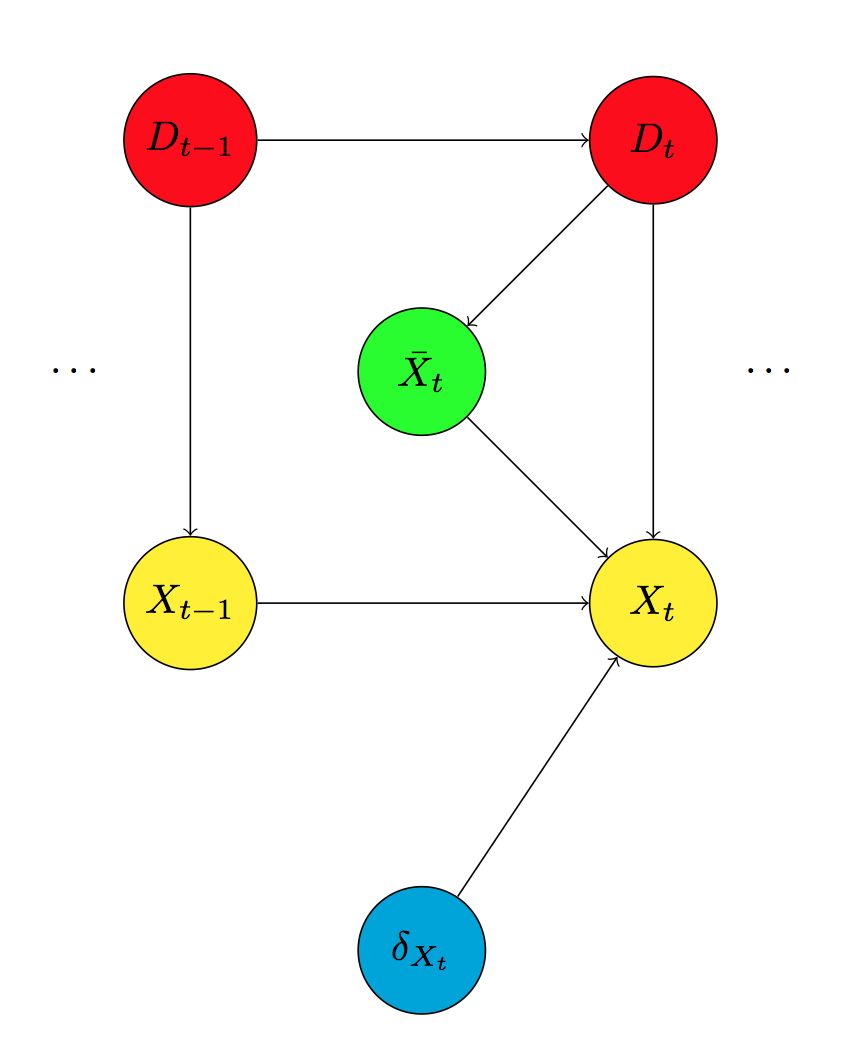
\includegraphics[scale=0.45]{./figures/CajaMarModel2}
\caption{Basic components of the DBN structure.}
\label{fig:component}
\end{center}
\end{figure}

\begin{figure}[htbp]
  \centering
   \begin{tabular}{cc}    
       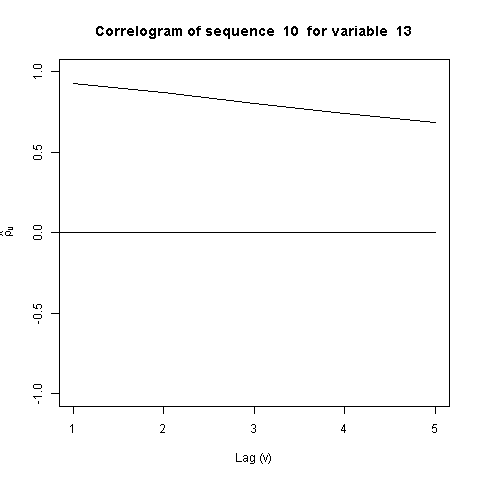
\includegraphics[width=70mm]{figures/CajamarCorrelogram} &
        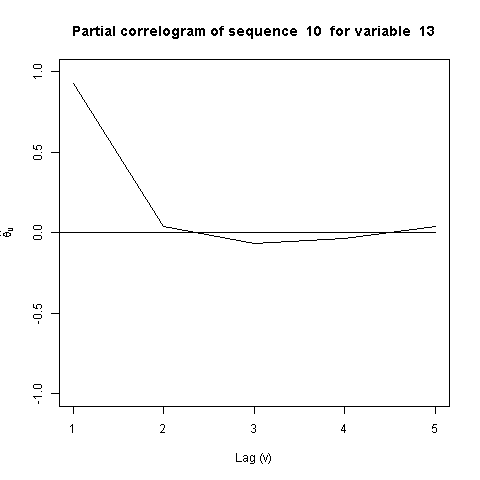
\includegraphics[width=70mm]{figures/CajamarPartialCorrelogram}
    \end{tabular}
     \caption{\label{fig:CajamarCorrelogramsAndPartial} Correlogram and partial correlogram for a variable. The x-axis represents the lag $v$ or time difference, and the y-axis represents the sample/partial autocorrelation coefficient of lag $v$, denoted $\hat{\rho_v}$ and $\hat{\delta_v}$, respectively (see Section \ref{Section:Preliminaries} for more details).}
\end{figure}

Another node included into the network in Figure \ref{fig:component} is the indicator variable $\delta_{X_t} \in \delta_{{\bf X}_t}$. This indicator variable is useful to model the situation in which a variable $X_t$ has a large number of zeroes, which is frequently encountered in Cajamar data. This is the case for variables whose corresponding events do not occur every day. For instance, every day payments made by credit card or the historical monthly outstanding amount on the account, whose value can be equal to zero for a large number of days for most customers. This fact can seriously affect learning, because the real behavior of $X_t$ for values different from 0 is not adequately captured by the learnt distribution.
The solution we propose is to use the indicator variable to condition the value of variable $X_t$ to $\delta_{X_t} = 0$ and $\delta_{X_t}\neq 0$. The indicator variables are not linked through consecutive time steps, as they are only used to indicate which data we model in the corresponding variable $X_t$. To better illustrate this, Figure \ref{fig:CajamarZeroes} (left) displays the histogram of a variable including all values, and Figure \ref{fig:CajamarZeroes} (right) displays the histogram of the same variable, but excluding all zero values. Note that the fitted density when zeros are discarded is extremely more representative than including zeros. This result undoubtedly justifies the use of the indicator variable $\delta_{X_t}$.

\begin{figure}[h]
  \centering
    \begin{tabular}{cc}    
       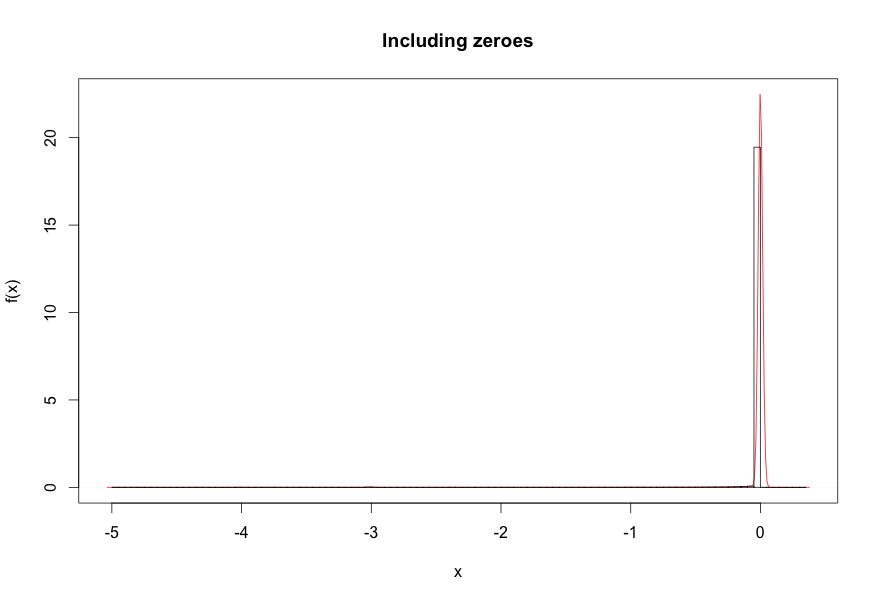
\includegraphics[width=70mm]{figures/with_zeroes}&
       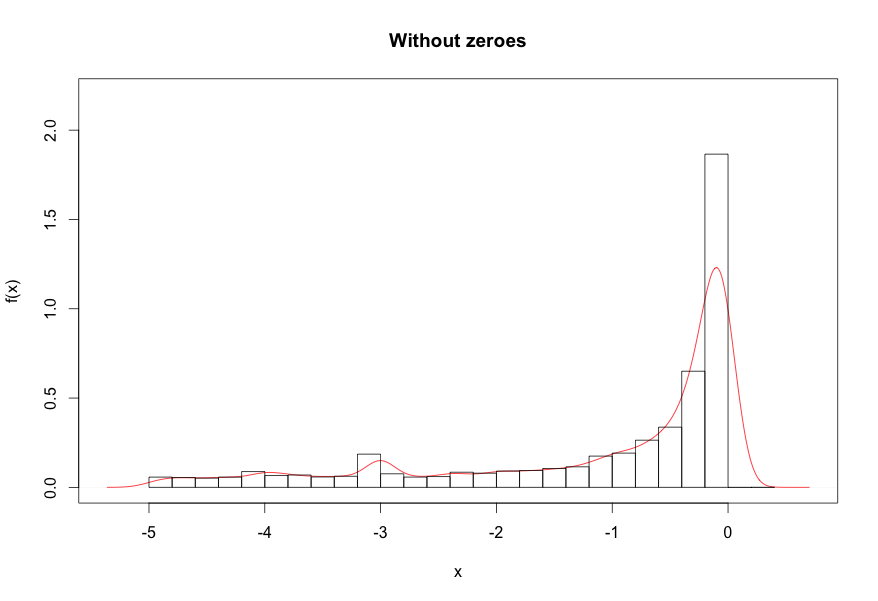
\includegraphics[width=70mm]{figures/without_zeroes}
    \end{tabular}
    \caption{\label{fig:CajamarZeroes}Data histograms and fitted densities for the same predictive variable including zeroes (left) and discarding them (right). In both cases, outliers have been removed for a clearer representation.}

\end{figure}

Finally, there exist some variables for which, even though some dependences over time would be expected, no dynamic behaviour is encountered. For instance, this is the case for variables\footnote{For confidentiality reasons, the names of the variables cannot be revealed.} whose correlograms, shown in Figure \ref{fig:cajamarCorr}, indicate values very close to zero for all lags. These variables are hence not linked through consecutive time steps in the dynamic model, and are represented by ${\bf Y}_{t}$ and  ${\bf Y}_{t+1}$. Moreover, static variables, denoted as $\Z$ in Figure~\ref{fig:CajamarStaticModel}, are also included in these groups with the only problem that their distributions must be replicated at times $t$ and $t+1$. 


\begin{figure}[h]
  \centering
    \begin{tabular}{cc}
    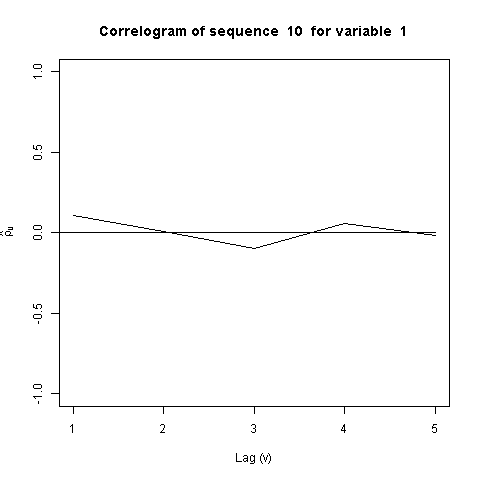
\includegraphics[width=70mm]{figures/CajaMarcrl1}&
     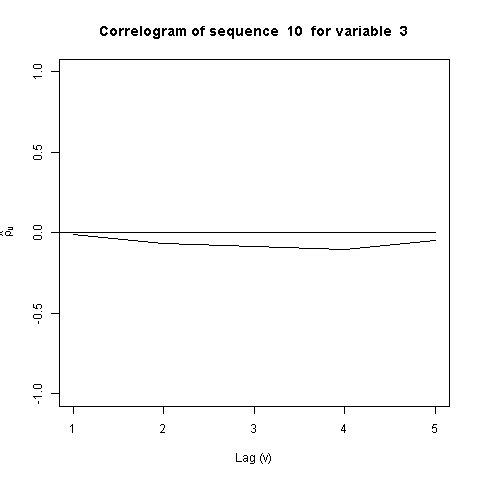
\includegraphics[width=70mm]{figures/CajaMarcrl3}\\
  \end{tabular}
    \caption{\label{fig:cajamarCorr}Example of correllograms for two predictive variables.  The x-axis represents the lag $v$ or time difference, and the y-axis represents the sample autocorrelation coefficient of lag $v$, denoted $\hat{\rho_v}$ (see Section~\ref{Section:Preliminaries} for more details).}
\end{figure}

In summary, although the dynamic model is different from the static one, the whole process of building the model from the original relational database and updating the customers risk is exactly the same as for the static case.

%-------------------------------------------------------------------------------------------------------
\subsubsection{Low risk profile extraction} \label{subsubsec:profileExtraction}
%-------------------------------------------------------------------------------------------------------

The main contribution of the project to the profile extraction aims at refining the number of targeted clients for a campaign by discarding non-solvent customers (i.e. clients with high probability of defaulting) that might be included using the existing models. Note that a small improvement in the process, can mean a great saving when launching the campaign. 

As commented above, when the marketing department launches a marketing campaign, they provide some restrictions over a subset of variables, which are denoted here by $\Z$, to be satisfied by the targeted clients.  Considering these restrictions, our proposal to refine initial set of targeted clients will be focused on obtaining good profiles based on specific inferences over the BNs built in the previous application scenario. Firstly, they will select a different subset of predictive variables $\Y$ also considered relevant when computing the final profile of the specific campaign. Mainly  socio-demographic variables will take part in this set, for example, the age of a client is a relevant predictor when designing campaigns to attract customers for a death insurance. 

If we denote the \emph{Defaulter} variable as $D$,  the objective is to compute the assignment $\Y = \y^{*}$ that has maximum a posteriori probability (MAP) given the evidence $D=$ \texttt{no}, and also given the restrictions to be satisfied by the clients, $\Z=\z$. These restrictions will be considered as \textit{soft evidence} during the inference process, meaning that fully specific evidence about all the variables might not be provided. For instance, the restriction for some continuous variables might state that the MAP assignment must be inside an specific interval.

Thus, the MAP operation is defined as follows:

\begin{equation}
\y^{*} = \underset{\y\in\Omega_{\Y}} {\mathrm{arg\,max}} ~ P(\Y=\y\mid D = \texttt{no}, \Z=\z)\, .
\label{eq:MAP}
\end{equation}

Note that the MAP operation will be performed over a model containing the whole set of variables (i.e. the variables in $\Y$ and $\Z$, and the rest non-relevant variables.) There is an open issue when performing MAP inference within continuous domains, because it implies the specification of the intervals of the continuous variables conforming the MAP assignments. This issue is further considered in the discussion section. 

Consider a simple example in which three predictors $\Y = \{ \emph{Age}, \emph{Marital Status}, \emph{Gender}\}$ are considered relevant to identity target customers for a \textit{death insurance} campaign. Consider also the restriction $\Z = \{Age>50\}$, which encodes the initial group of customers that, according to the knowledge of the marketing group, are potential buyers of this product.  The next step is to further refine this group of customers and identify the profile of customers which are most solvent (i.e. less likely to default). After computing Eq.~\ref{eq:MAP}, this may result in the following most probable assignment: clients in the range \emph {[60-70] years}, \emph{single status} and \emph{male}. Hence, this profile identifies the most solvent customers who might be interested in purchasing a \emph{death insurance} product. We must say that the above  procedure could be also used to get the $k$ assignments with the highest posterior probability or, in other words, the best set of profiles.   

%With the solution presented above, Cajamar plans to reach higher benefits in credit operations starting from a campaign rather than directly from regular credit operations.  

%-------------------------------------------------------------------------------------------------------
%\subsubsection*{Static model}\label{sec:StaticModel}
%-------------------------------------------------------------------------------------------------------

As pointed out before, mainly socio-demographic variables will determine the customer profiles used in the campaigns. These variables are mostly static, as they do not change frequently over time (e.g., marital status, gender, type of job, ...). However, to enhance the analysis, a number of  variables changing over time will be included. 
%Note that this does not mean the use of a dynamic model.

%Due to complexity reasons, we should reduce this number as much as possible to make the profile extraction problem feasible.
The BN model used for the profile extraction will be, in a first attempt, the same static model that was used for predicting the risk of defaulting (see Figure~\ref{fig:CajamarStaticModel}). However, there will be a considerable reduction in the number of features included, since the profile extraction task does not require information about all variables included in the risk prediction, i.e., only a few variables will be part of the profiles. With this reduction, we also make the problem computationally more feasible. I.e. In this first attempt only variables within each white box (see Figure~\ref{fig:CajamarStaticModel}) will be allowed to be connected by conforming a tree structure. 

In Section~\ref{subsubsec:CajamarDiscussion} we will discuss the possibility of considering models with more dependences among white boxes, and also having a general Bayesian network structure more than one specifically designed for classification. Mainly, because for MAP inferences is desirable to avoid na\"{\i}ve-Bayes-type structures like the one of the static model of Figure~\ref{fig:CajamarStaticModel}. The reason is that, once the \emph{Defaulter} variable is evidenced to \texttt{no}, the features become independent and the analysis would be poorer (the MAP solution in this case would correspond to the maximum probability value for each variable individually).

The use of this static BN model commented above should be considered as a baseline model. We expect that the employment of alternative dynamic models will give us further improvements in the performance of this MAP based approach. An extension including dynamic Bayesian networks is further discussed in the next section.

%-------------------------------------------------------------------------------------------------------
%\subsubsection*{Dynamic model}
%-------------------------------------------------------------------------------------------------------

 
%-------------------------------------------------------------------------------------------------------
\subsubsection{Discussion and future models}\label{subsubsec:CajamarDiscussion}

%-------------------------------------------------------------------------------------------------------
%\textcolor{red}{Should we discuss something about overfiting  in Figure 4.17?}

The static and dynamic models presented above for the two tasks represent a first attempt to address the Cajamar use case. In this section, we will discuss the potential modifications and/or extensions that may occur in the subsequent phases of the AMIDST project to better meet Cajamar requirements presented in~\cite{Fer14b} or to face, for instance, other unexpected events. This discussion is also essential as we are still considering expert advice that could slightly modify some of proposals as the project moves forward.

The static model shown in Figure~\ref{fig:CajamarStaticModel} for predicting the probability of default is assumed to have only dependences among variables within each group of variables (white boxes). However, according to expert knowledge, no limitations should be imposed to the model structure among the predicting variables. Figure~\ref{fig:staticDependences} shows the modified structure of the static model when dependences among predicting variables are allowed, meaning that, variables within the dashed blue box could be connected as well. Note that, in this case, complexity grows considerably but, it is worth considering this approach to capture dependences that intuitively are not expected and, therefore, the analysis will be enriched.

\begin{figure}[ht!]
  \centering
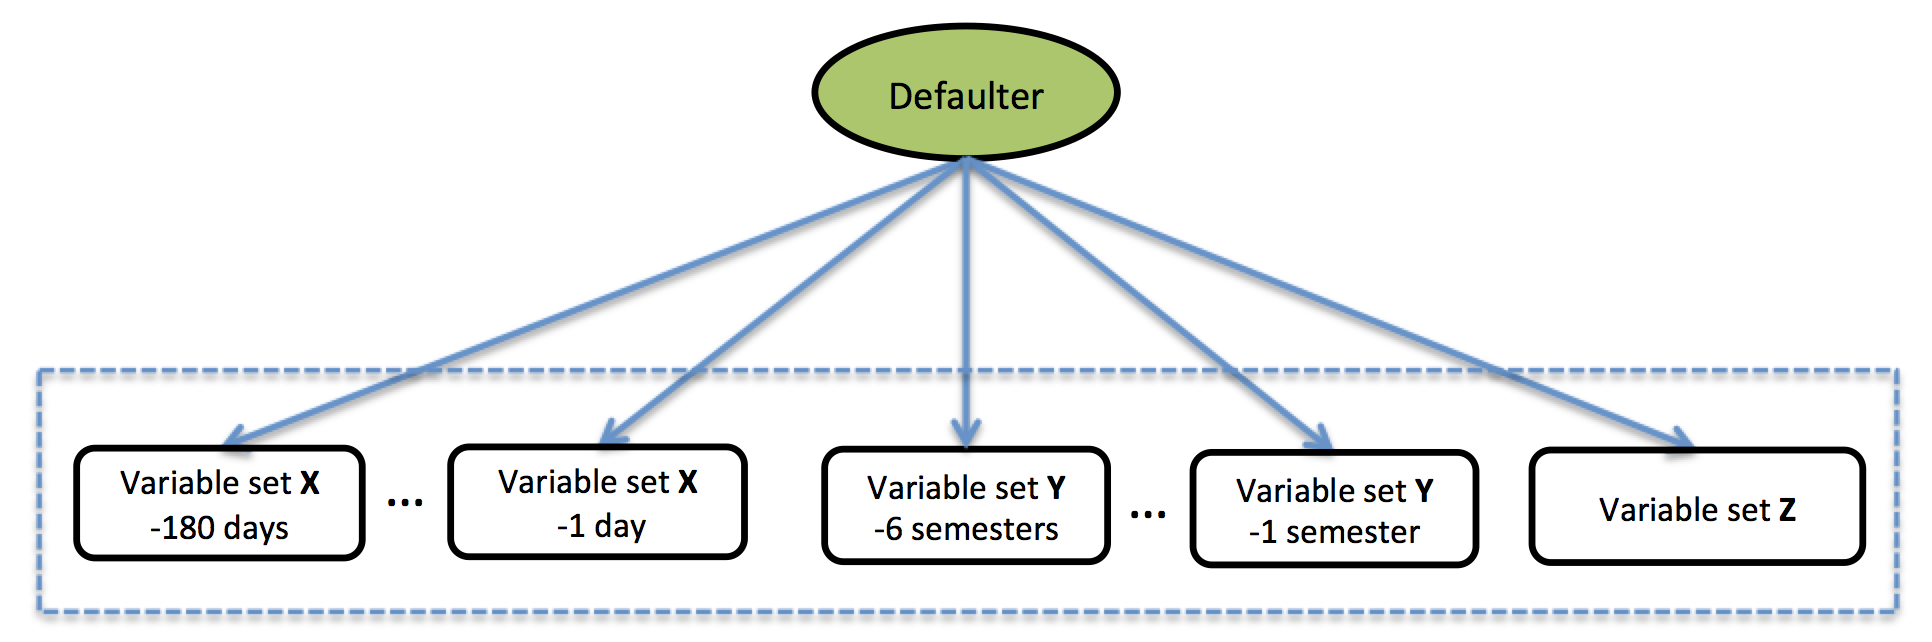
\includegraphics[scale=0.4]{./figures/CajaMarModel3}
\caption{\label{fig:staticDependences}Global structure of the static model allowing dependences among any variable within the dashed blue box. Each white box represents a set of variables for a particular time. The green node on top is the class variable \emph{Defaulter} that represents the probability that a customer will default within the next two years.} 
\end{figure}

In general, the model structure in Figure~\ref{fig:staticDependences} can not be modeled by CG distributions if discrete children happen to have continuous parents (see Section~\ref{SubSection:HybridBNs}). If so, other probability distributions families will be explored. Mainly, they consist in translating the probability distribution into another such that learning and inference become feasible. These approaches include discretization or more complicated families based on Mixture of Truncated Basis Functions~\cite{Langseth12}, which can cope with any generic model structure.

There is another open issue about the complexity of the profile extraction task explained in Section~\ref{subsubsec:profileExtraction}. It is well known that MAP inference over BNs is an NP-hard problem~\cite{Shi94}. Thus, the model presented in Figure~\ref{fig:staticDependences}, which is valid for the profile extraction as well, could be simplified if necessary by manually reducing the number of predictors in such a way that computational burden is adapted to the needs. In fact, this process is tightly connected to the expert knowledge provided by the marketing group, and this refinement should not encounter major difficulties. Moreover, we could consider having a general Bayesian network structure instead of one specifically designed for classification. In this way, dependences among the features included in the profiles might be modelled without the restrictions imposed in classification based structures.

The model for predicting the risk of default is assumed to be learnt every day. However, if required, this assumption can be relaxed and the learning process could be carried out less frequently. The results hardly will be affected as one-day data have little impact in comparison with the historical data captured in the current model so far. Note that, even if the model is not updated, the risk predictions are computed every day using the latest model available so far.

%\textcolor{red}{Are we going to use a dynamic model for the profile extraction problem (to be decided)? If so, how MPE inference is performed in a dynamic BN? Which node is evidenced Defaulter(t) or Defaulter(t+1)? What does MPE means in this case?} 
An extension of the static model proposed in Section~\ref{subsubsec:profileExtraction} for the profile extraction would involve not only considering those variables evolving over time, but also their tendency by using a dynamic Bayesian network. Initially, the model for the profile extraction will be the same as the one depicted in Figure~\ref{fig:component} but with a considerable reduction in the number of predictors as in the static case. With this model, the MAP solution could capture temporal trends in the customer profiles. 

Finally, as commented above, there is an open issue when performing MAP inference within continuous domains, which is the definition of the intervals of the continuous variables conforming the MAP solution. A first approach could be to discretize the continuous variables and then use the corresponding intervals to defineº the profiles. 





